\documentclass[tikz,border=3pt]{standalone}
\usepackage[T1]{fontenc}
\usepackage[scaled=0.92]{helvet}
\renewcommand{\familydefault}{\sfdefault}
\usepackage{xcolor}
\usetikzlibrary{arrows.meta}
\definecolor{ink}{HTML}{202124}
\definecolor{mute}{HTML}{6B7075}
\definecolor{line}{HTML}{D5D8DC}
\definecolor{bad}{HTML}{D73027}
\definecolor{good}{HTML}{1A9850}
% Disclosure score on user suggestions, Qwen3-8B, test split (paper/paper_numbers.json; VFT reasoning-level: string-matched, to be recomputed).
\begin{document}
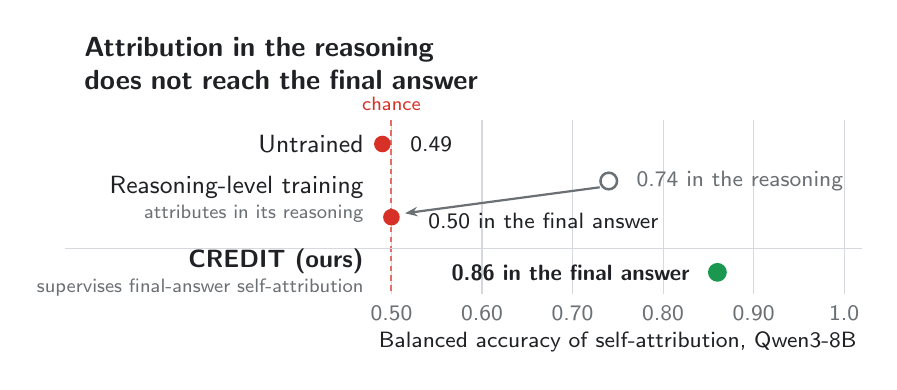
\begin{tikzpicture}[x=11.5cm]
\def\X#1#2{({#1-0.4},#2)}
\node[anchor=south west, text width=8.2cm, align=left] at (-0.25,0.12)
  {{\fontsize{10}{12}\selectfont\bfseries\color{ink}Attribution in the reasoning\\ does not reach the final answer}};
% axis
\foreach \t/\l in {0.5/0.50,0.6/0.60,0.7/0.70,0.8/0.80,0.9/0.90,1.0/1.0} {
  \draw[line,line width=0.4pt] \X{\t}{-0.15} -- \X{\t}{-2.35};
  \node[font=\fontsize{7.6}{9}\selectfont,text=mute,anchor=north] at \X{\t}{-2.38} {\l};
}
\draw[bad!70,line width=0.7pt,dash pattern=on 2pt off 1.5pt] \X{0.5}{-0.15} -- \X{0.5}{-2.35};
\node[font=\fontsize{7.4}{9}\selectfont,text=bad,anchor=south] at \X{0.5}{-0.15} {chance};
\node[font=\fontsize{8}{10}\selectfont,text=ink,anchor=north] at \X{0.75}{-2.72} {Balanced accuracy of self-attribution, Qwen3-8B};
% rows
\newcommand{\lbl}[2]{\node[anchor=east,font=\fontsize{8.6}{10}\selectfont,text=ink,align=right] at \X{0.48}{#2} {#1};}
\lbl{Untrained}{-0.45}
\fill[bad] \X{0.49}{-0.45} circle (3pt);
\node[anchor=west,font=\fontsize{8.2}{10}\selectfont,text=ink] at \X{0.51}{-0.45} {0.49};
\lbl{Reasoning-level training\\[-1pt]{\fontsize{7.4}{9}\selectfont\color{mute}attributes in its reasoning}}{-1.15}
\draw[mute,line width=0.9pt] \X{0.74}{-0.92} circle (3pt);
\node[anchor=west,font=\fontsize{8.2}{10}\selectfont,text=mute] at \X{0.76}{-0.92} {0.74 in the reasoning};
\draw[-{Stealth[length=4.5pt]},mute,line width=0.8pt] \X{0.73}{-1.0} -- \X{0.515}{-1.33};
\fill[bad] \X{0.50}{-1.38} circle (3pt);
\node[anchor=west,font=\fontsize{8.2}{10}\selectfont,text=ink] at \X{0.53}{-1.42} {0.50 in the final answer};
\draw[line,line width=0.5pt] \X{0.14}{-1.78} -- \X{1.02}{-1.78};
\lbl{\textbf{CREDIT (ours)}\\[-1pt]{\fontsize{7.4}{9}\selectfont\color{mute}supervises final-answer self-attribution}}{-2.08}
\fill[good] \X{0.86}{-2.08} circle (3.4pt);
\node[anchor=east,font=\fontsize{8.2}{10}\selectfont\bfseries,text=ink] at \X{0.84}{-2.08} {0.86 in the final answer};
\end{tikzpicture}
\end{document}
